\documentclass[12pt,fleqn]{article}
\usepackage{xiiiemc}
\usepackage{natbib}
\usepackage{fancyhdr}
\usepackage{color}
\usepackage{wallpaper} 
\usepackage{titlesec}   %% Define space between paragraph e section
\usepackage{float} 	%% Use to fix Figure or Table: ex: \begin{table}[H]
%%%%Don't edit this block. It reduces the spacing between the lines of the references
\let\OLDthebibliography\thebibliography
\renewcommand\thebibliography[1]{\OLDthebibliography{#1} \setlength{\parskip}{0pt}\setlength{\itemsep}{0pt plus 0.3ex}}

%%-----------------------------------------------EDIT-----------------------------------------------
\title{TEXT MINING DESCRIPTIONS OF DREAMS: AESTHETIC AND THERAPEUTIC EFFORTS}

%%-----------------------------------------------EDIT----------------------------------------------
\author
    {\rm \begin{tabular}{l} 
    \textbf{Renato Fabbri}$^{1}$ - {\textnormal renato.fabbri@gmail.com}\\%
    \textbf{Fabiane M. Borges}$^{2}$ - {\textnormal catadores@gmail.com}\\
    {\fontsize{11}{0}\selectfont $^{1}$University of São Paulo, Institute of Mathematical and Computer Sciences - São Carlos, SP, Brazil}\vspace*{-0.05cm} \\
    {\fontsize{11}{0}\selectfont $^{2}$Federal University of Rio de Janeiro, School of Fine Arts - Rio de Janeiro, RJ, Brazil}\vspace*{-0.05cm}\\
  \end{tabular}}
%%----------------------------------------------------------------------------------------------

\fancypagestyle{firspagetstyle}
{
	\lhead{}
	\fancyhead[C]{%
		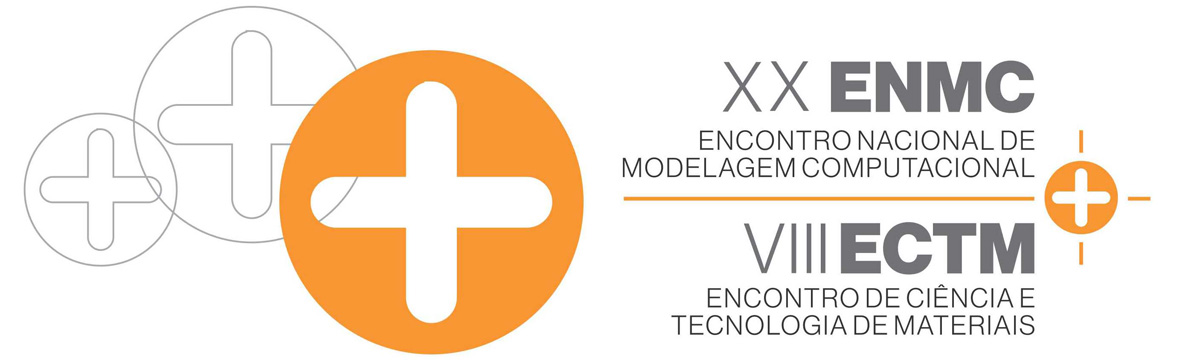
\includegraphics[width=0.9\linewidth]{logo}\\%
		{\scriptsize \fontfamily{phv}\fontseries{b}\selectfont \color[rgb]{0.45,0.45,0.45}
		16 a 19 de Outubro de 2017\\
		Instituto Politécnico - Universidade do Estado de Rio de Janeiro\\
		Nova Friburgo - RJ\\
	    }
	}
	\renewcommand{\headrulewidth}{0.0pt}
	\fancyfoot[C]{\footnotesize \parbox{15cm} {\centering  \fontsize{7.5}{0}\selectfont \it Anais do XX ENMC – Encontro Nacional de Modelagem Computacional e VIII ECTM – Encontro de Ciências e Tecnologia de Materiais,  Nova Friburgo, RJ – 16 a 19 Outubro 2017}} % \ttfamil
	\rhead{}
}


\begin{document}
\maketitle

\thispagestyle{firspagetstyle}

\fancyhead[L]{\footnotesize{\fontsize{7.5}{0}\selectfont \it XX ENMC e VIII ECTM\\
	16 a 19 de Outubro de 2017\\
	Instituto Politécnico Universidade do Estado do Rio de Janeiro – Nova Friburgo - RJ\\}}
\renewcommand{\headrulewidth}{0.0pt}
\fancyfoot[C]{\footnotesize \parbox{15cm} {\centering  \fontsize{7.5}{0}\selectfont \it Anais do XX ENMC – Encontro Nacional de Modelagem Computacional e VIII ECTM – Encontro de Ciências e Tecnologia de Materiais,  Nova Friburgo, RJ – 16 a 19 Outubro 2017}} % \ttfamil
\rhead{}

\begin{abstract}
	Dreams are highly valued in both Freudian psychoanalysis and less conservative therapeutic traditions.
	Text mining enables the extraction of meaning from writings in powerful and unexpected ways.
	In this work, we report methods, uses and results obtained by mining descriptions of dreams.
	The texts were collected as part of clinical practices from dozens of volunteers.
	They were subsequently mined using various techniques for the achievement of poems and summaries,
	which were then used in schizoanalysis (therapeutic) sessions by means of music and declamation.
	The results were found aesthetically appealing and effective to engage the audience of patients.
	The expansion of the corpus, mining methods and strategies for using the derivatives for art
	and therapy are considered for future work.
\end{abstract}

\keywords{\em{Dreams, Text mining, Poetry, Art, Schizoanalysis}}

\pagestyle{fancy}

\section{INTRODUCTION}
Although dreams are described in texts that range from ancient sacred~\cite{bible}
to recent medical~\cite{dreamMed}, there is no consensus of what dreams are.
We can exemplify the diverse theories with three simple cases:
\begin{itemize}
	\item Dreams are often regarded by the dreamers as accessing spiritual helms or other realities.
	\item Many scientists regard dreams as by-products of the sleeping process:
		arbitrary interpretations given by the conscious mind to noisy signals without substantial meaning.
	\item Freudian and Jungian psychoanalysis traditions understand dreams as symbolic constructs output by the unconscious mind.
\end{itemize}
\noindent We can, however, state some facts about dreams that make them very interesting material for therapy and for art.
First, dreams are often very rich in impacting and symbolic images.
Second, they are told by the person who dreamed in a very attentive manner, as being very significant to the dreamer.
In fact, most of us should be able to remind of a number of situations where someone (perhaps ourselves)
was describing a dream in a rapid, almost euphoric, succession of words.
Dreams are so effective in yielding artistic materials that surrealism is an aesthetic explicitly inspired by dreams and
symbolism is an example of artistic movement heavily influenced by dreams.

Text mining is data mining applied to textual data.
There are many models for the text mining pipeline, but
it can be summarized as: data collection and preparation,
pattern recognition, evaluation of the output and reporting.
This work addresses text mining of descriptions of dreams
with aesthetics and therapeutic purposes.

Section~\ref{sec:matMet} describes the corpus and methods.
Section~\ref{sec:res} is dedicated to presentation and discussion of results.
Section~\ref{sec:conc} holds conclusions and further work considerations.

\section{MATERIALS AND METHODS}
\subsection{Corpus}
The description of dreams we used are~\cite{dreams1} all in Brazilian Portuguese,
collected as part of clinical practices in the year of 2014.
Volunteers described the dreams and sent them to the second author or this paper.
Thereafter, another collection of dreams~\cite{dreams2} was gathered in the same way by the second author,
with the purpose of expanding the analysis and synthesis of texts performed with the previous
corpus, but was not used until now.
It is a larger corpus, also in Brazilian Portuguese.
Interestingly, both corpus contains description of dreams by women only.
Both corpus are summarized in Table~\ref{tab:dreams} in numbers of dreams, paragraphs,
and letters.

\subsection{Analysis and derivation methods}
The texts were analyzed to support the extraction of meaning from the dreams
and for the creation of artistic texts.
We strived to keep the methods very simple in order to avoid puzzling the involved parties.
We considered three lists of tokens:
\begin{itemize}
	\item punctuations !"\#\$\%\&'()*+,-./:;<=>?@[]\textbackslash\textasciicircum\_`\{\}|\textasciitilde. Obtained through the command \\ \texttt{string.punctuation} of Python's string (standard) library.
	\item Portuguese \emph{stopwords}\footnote{The exact definition and list of stopwords are not consensual.
		Anyway, one can regard them as words with lesser meaning and which are very frequent, such as conjunctions and prepositions.}
		obtained through NLTK~\cite{nltk} by the command \\ \texttt{nltk.corpus.stopwords.words("portuguese")}.
	\item Tokens in the texts which were not punctuations nor stopwords.
		These were regarded as the most meaningful words in the text and were used in their order of appearance.
\end{itemize}

This list of most meaningful words was used as the core material for the achievement
of more interesting constructions for
art and therapy through filtering and ordering.
Most significantly, the ordering could be based on the alphabet, the size of tokens in number of letters,
or the count of incidences of the words, or any combination of these.
Filtering could be performed by restricting the vowels, consonants (e.g. fricatives), word size, frequency, or
collocations.

\section{RESULTS AND DISCUSSION}
The list of most meaningful words (described in the previous section) was filtered and ordered
in many ways to yield diverse sequences of interest.
After an inspection of the results, these criteria were selected to compose a final document:
\begin{itemize}
	\item Ordering by: incidence (most frequent words first),
alphabetic, size in characters, with and without repetitions.
These were considered the most raw sequences and used subsequently to derive other sequences
		with such variations of ordering and repetition.
	\item Words with only one vowel (repeated any number of times).
	\item Only words with fricatives or plosives or
some combination of them (e.g. plosives and m and vowels 'a' and 'e').
	\item Words that start and end sentences.
	\item Collocations (pair of words which are frequent).
\end{itemize}

Such final document and other files are available online and exposed in Table~\ref{tab:files}.
An example of these texts is in Table~\ref{tab:comecoFinal} with a translation
from Portuguese to English.
These texts were used for aesthetic appreciation and also in a schizoanalysis group session
in 2014, Casa Nuvem, Rio de Janeiro, RJ, Brazil.
The artist Giuliano Obici used the texts to make live electroacoustic music,
which was accompanied by declamations.
The groups was constituted by the volunteers who described the dreams and
the description of the episode is somewhat impressive:
the members had strong impressions, some of them cried and entered a quasi-shock state. 

\newpage %

\vspace{12cm}

\begin{table}[H] % !htbp 
	\caption{Example of artistic text obtained from description of dreams.
	This text was obtained through picking only the first and last words of each sentence.}\label{tab:comecoFinal}
\vspace{12pt}
\centering{}
\begin{tabular}{  c | c }
Escorregava glandes              &                                                Slipping glands         \\
Numa assustavam                  &                                                At once, they scared    \\
Eu suada                         &                                                I sweated               \\
As cavalos                       &                                                The horses              \\
Não acabou                       &                                                It's not over           \\
Barras mim                       &                                                Bars me                 \\
Andei construtores               &                                                I walked builders       \\
Pessoas )                        &                                                People  )               \\
Sonhei formei                    &                                                I dreamed I formed      \\
Estava menino                    &                                                It was boy              \\
Depois boa                       &                                                Then good               \\
Esse meu                         &                                                This mine               \\
Sonhos descendo                  &                                                Dreams coming down      \\
O irmão                          &                                                The brother             \\
Meu punição                      &                                                My punishment           \\
Começa irmão                     &                                                Begins brother          \\
Meu ele                          &                                                My him                  \\
Meu demonstração                 &                                                My demonstration        \\
Depois ”                         &                                                After "                 \\
Eu parede                        &                                                I wall                  \\
Sinto dele                       &                                                I'm fell him            \\
A importência                    &                                                The ``importence''      \\
O buraco                         &                                                The hole                \\
Acordei ofegante                 &                                                Woke up breathless    \\
Sensação NÃO                     &                                                Feeling NO              \\
Já rumo                          &                                                I'm on my way           \\
Estava perseguido                &                                                Was persecuted          \\
Quando percebeu                  &                                                When realized    \\
A tempo                          &                                                In time                 \\
Até porta                        &                                                Up to door              \\
O disso                          &                                                The this                    \\
Eu sobreviver                    &                                                I survive               \\
\end{tabular}
\end{table}

\newpage %

% \newpage %
\section{CONCLUSIONS AND FUTURE WORK}
We understand that the results are compelling for both art and therapy.
Only the first corpus was used, which is smaller and made easier the selection of the resulting texts.
The methods applied are very simple, favoring the communication between the parties,
and are promptly deepened and expanded into more complex processes.
This work seems unique in the sense of using text mining of dreams for art and therapy,
which, in our opinion, benefit the appreciation of it as a multidisciplinary scientific contribution
in computer science, art and psychology (schizoanalysis).

In further efforts,
we might use for the corpus:
\begin{itemize}
	\item descriptions of dreams in the literature (e.g. Bible);
	\item other languages;
	\item an expansion of current corpus;
	\item dreams from specific groups, e.g. again gender related or of a specific age span, professional or educational background, etc.
\end{itemize}

\noindent About the text mining methods, we might:
\begin{itemize}
	\item Use specific routines for classification (e.g. clusterization) of texts or their features.
	\item Expand the methods of selection of words to better encompass meter (e.g. number of syllables).
	\item Expand methods of selection of words and phrases by their sonorities: sequence of vowels or consonants, mute consonants, paroxytones, etc.
	\item Use Wordnet in order to relate terms through semantic links (e.g. hypernymy, meronymy, synonymy).
\end{itemize}

The exploration of the results in therapeutic sessions and for the achievement of compelling selections of
artistic texts should be kept as the core purposes.

\subsection*{\textit{Acknowledgements}}
The authors thank the volunteers who supplied the descriptions of dreams;
the subjects with attended to the schizoanalysis sessions;
the open source software developers, especially those who enabled this work by developing
the Python language and the NLTK.

% ------------------------------------------------------------------------
\begin{thebibliography}{99}
\fontsize{11}{0}\selectfont
\bibitem[Aznar \& Pessoa, 1994]{Aznar94}
Aznar, M., Pessoa, F.L.P. and Silva Telles, A. (1994), ``Vapor-Liquid Equilibria of Mixed Solvent-Salt Systems using a MHV2 Model with the Wilson Equation'', {\em X Congresso Brasileiro de Engenharia Química}, São Paulo, vol 1, 38-43.

\bibitem[Freitas et~al., 2008]{Freitas08}
de Freitas, G.C.S.; Peixoto, F.C.; Vianna Jr, A.S. (2008), Simulation of a thermal battery using Phoenics. Journal of Power Sources, 179, 424-429. 

\bibitem[Duarte, 1999]{Duarte99}
Duarte, C.S.A. (1999), {\em Equilíbrio Líquido-Líquido em Sistemas contendo Polímero e Eletrólito: Água/ Polietileno-glicol/Fosfato}, Laboratório de Equilíbrio de Fases, FEQ/UNICAMP, Campinas.

\bibitem[Fredenslund, 1993]{Fredenslund93}
Fredenslund A. e Sorensen, J.M. (1993), ``Group Contribution Estimation Methods'', in {\em  Models for Thermodynamic and Phase Equilibria Calculations}, S.I. Sandler (ed.), Marcel Dekker, Inc., New York.

\bibitem[Silva, 2005]{Silva2005}
Silva, L.F. (2005), ``{\em Predição de Pontos Críticos de Misturas Termodinâmicas}'', Tese de Doutorado, IPRJ/UERJ, Nova Friburgo.

\bibitem[Krevelenm, 1990]{Krevelen90}
Van Krevelen, D.W. (1990),{\em ``Properties of Polymers. Their Correlation with Chemical Structure, Their Numerical Estimation and Prediction from Additive Group Contribuition}'', 3º ed., Elsevier, Amsterdam.
\end{thebibliography}
\vspace*{-0.1cm}
\section*{APPENDIX A}
This section, if necessary, must be included here.

\vspace{0.5cm} % Example spaces

For Papers written in Portuguese or Spanish a translation of title, abstract and keywords into English must be provided after the Appendix using the same format for title, abstract and keywords presented in the first page of the template.
% ------------------------------------------------------------------------

%For papers written in Portuguese or Spanish.

%\begin{center}
%  TITLE IN ENGLISH
%\end{center}

%\def\abstractname{Abstract}%

%\begin{abstract}
%   Abstract in english
%\end{abstract}

%\keywords{\em{Keywords in english}}

\end{document}
